% LeadMate Capstone Project Report
% Build: pdflatex (recommended: xelatex)
\documentclass[11pt,a4paper]{report}

% Packages
\usepackage[utf8]{inputenc}
\usepackage[T1]{fontenc}
\usepackage{lmodern}
\usepackage{newtxtext,newtxmath}
\usepackage{geometry}
\usepackage{setspace}
\usepackage{graphicx}
\usepackage{adjustbox}
\usepackage{hyperref}
\usepackage{booktabs}
\usepackage{longtable}
\usepackage{listings}
\usepackage{xcolor}
\usepackage{amsmath}
\usepackage{caption}
\usepackage{subcaption}
\usepackage{tikz}
\usetikzlibrary{arrows.meta,positioning,shapes,calc}
\usepackage{adjustbox}
\usepackage{enumitem}
\usepackage{multirow}
\usepackage{array}
\usepackage{pgfplots}
\pgfplotsset{compat=1.17}
\usepackage{pgfgantt}
\setlist{nosep}

\geometry{margin=1.25in}
\raggedbottom
\setlength{\parskip}{0.6em}
\setlength{\emergencystretch}{2em}
\onehalfspacing
\hypersetup{colorlinks=true,linkcolor=blue,citecolor=blue,urlcolor=blue}
% Longtable tuning for page fit and readability
\setlength{\LTcapwidth}{\textwidth}
\setlength{\LTleft}{0pt}
\setlength{\LTright}{0pt}
\AtBeginEnvironment{longtable}{\small}

% Metadata
\title{LeadMate: AI-Driven Team Lead Assistant for Project Understanding, Stack Decisions, and Team Formation}
\author{LeadMate Team}
\date{\today}

% Code listing style
\lstdefinestyle{code}{
  basicstyle=\ttfamily\small,
  breaklines=true,
  tabsize=2,
  keywordstyle=\color{blue},
  commentstyle=\color{gray},
  stringstyle=\color{teal}
}

\begin{document}

\pagenumbering{roman}
\begin{titlepage}
  \centering
  \vspace*{6mm}
  {\Large \textbf{Woxsen University, School of Technology}\\[2mm]}
  {\large Department of Computer Science and Engineering}\\[10mm]
  % Logo
  \IfFileExists{assets/woxsen_logo.png}{\includegraphics[height=25mm]{assets/woxsen_logo.png}}{\fbox{Woxsen University Logo}}\\[10mm]
  % Title
  {\LARGE \textbf{LeadMate: AI-Driven Team Lead Assistant for Project Understanding, Stack Decisions, and Team Formation}\\[8mm]}
  % Students and Guide
  {\large\textbf{Student(s):} Sanjay (Roll No.), Nikunj (Roll No.), Vastav (Roll No.)\\[3mm]}
  {\large\textbf{Guide/Faculty:} Dr. Faculty Name, Associate Professor}\\[8mm]
  % Academic Year & Semester
  {\large Academic Year: 2025--2026 \hspace{8mm} Semester: 7th}\\[15mm]
  % Footer
  \vfill
  {\large \today}
\end{titlepage}
\begin{abstract}
LeadMate is a full-stack, AI-assisted platform that helps engineering managers and team leads rapidly understand project documentation, analyze live repositories, recommend technology stacks, and form effective teams. The system integrates a FastAPI backend with modular routers, MongoDB for persistence, ChromaDB and optional MongoDB Atlas Vector for retrieval, and CrewAI agents orchestrated with Gemini (fallback to Ollama). A React + Vite frontend provides protected role-based workflows for managers and team leads. This report presents the problem framing, related work, system design, implementation, evaluation, and an MVP with roadmap.
\end{abstract}

\tableofcontents
\listoffigures
\listoftables

\chapter*{Acknowledgements}
\addcontentsline{toc}{chapter}{Acknowledgements}
We thank contributors for architecture, implementation, and documentation support across backend, services, agents, and the React frontend.

\chapter{Introduction}
\pagenumbering{arabic}
\section{Problem Statement}
Engineering managers and team leads face fragmented data across PDFs, slide decks, wikis, source repositories, and ad-hoc resumes. Turning these artifacts into a coherent understanding of the project scope, constraints, and staffing plan is time-consuming and error-prone. LeadMate addresses this gap with an integrated system for ingesting and structuring artifacts, enabling retrieval-augmented question answering (RAG), and orchestrating specialized agents to propose technology stacks and team compositions grounded in the project's context.

\section{Objectives}
\begin{itemize}
  \item Automate document analysis and Q\&A grounded in project context.
  \item Analyze real Git repositories for activity, quality, and trends.
  \item Recommend technology stacks and team compositions with justification.
  \item Provide a manager/lead-friendly UI with role-based access control.
\end{itemize}

\section{Scope}
LeadMate covers document ingestion (PDF, DOCX, text), chunking and vectorization, contextual chat over documents, repository analytics with insights, and agentic recommendations for technology stack and team formation. Out of scope are budgeting, sprint management, and vendor procurement; these may consume LeadMate outputs but are not implemented within the platform.

\chapter{Literature Review and Background}
\section{RAG and Vector Stores}
LeadMate employs a two-tier information retrieval approach. By default, documents are chunked and embedded into project-scoped ChromaDB collections for low-latency semantic search. A deployment variant can instead use MongoDB Atlas Vector Search, storing chunks and embeddings alongside document metadata to simplify operational management. Both strategies support grounded responses by constraining the LLM to project-specific evidence.

\section{Agent Orchestration}
CrewAI coordinates specialized agents with clear roles. The Document Agent focuses on Q\&A and summarization; the Stack Agent translates requirements into FE/BE/DB/cloud recommendations; the Team Formation Agent proposes role mixes based on scope, timelines, and available resumes. Gemini provides primary LLM capabilities with a runtime fallback to Ollama for offline or cost-sensitive environments.

\section{Comparable Systems}
Developer copilots and knowledge bases provide adjacent capabilities, but LeadMate unifies documents, repos, and team formation in one flow.

\section{Background Information}
Relevant domain knowledge includes software project documentation practices, developer workflow analytics, and organizational design principles. Industry trends favor hybrid retrieval-generation pipelines and model orchestration.

\section{Significance and Scope}
This project focuses on practical value: faster onboarding, risk-aware decisions, and staffing clarity. It excludes budgeting and sprint tracking by design.

\section{Gap Analysis}
Table~\ref{tab:related-work} compares LeadMate against representative tools across capabilities.
\begin{longtable}{p{3.2cm}p{2.2cm}p{2.2cm}p{2.2cm}p{5.2cm}}
\caption{Related work comparison}\label{tab:related-work}\\
\toprule
\textbf{System} & \textbf{Doc RAG} & \textbf{Repo Analytics} & \textbf{Team Formation} & \textbf{Notes}\\
\midrule
\endfirsthead
\toprule
\textbf{System} & \textbf{Doc RAG} & \textbf{Repo Analytics} & \textbf{Team Formation} & \textbf{Notes}\\
\midrule
\endhead
LeadMate (this work) & Yes & Yes & Yes & Unified flow and shared context across agents.\\
Generic Copilot & Limited & No & No & Inline coding aid; lacks org context and PM signals.\\
Knowledge Base + Q\&A & Yes & No & No & Strong RAG; no engineering activity integration.\\
Dev Analytics Platform & No & Yes & No & Metrics dashboards; no LLM-grounded reasoning.\\
\bottomrule
\end{longtable}

\chapter{System Requirements}
\section{Functional Requirements}
\begin{itemize}
  \item Upload and parse project documents and resumes.
  \item Synchronize chunks and embeddings for fast semantic search.
  \item Chat/Q\&A over project context (DocAgent).
  \item Analyze Git repos and produce insights.
  \item Recommend stack and propose team roles (StackAgent, TeamFormationAgent).
\end{itemize}

\section{Non-Functional Requirements}
\section{Technology Review Summary}
The chosen stack balances operational simplicity with performance. ChromaDB supports local development with predictable latency; Atlas Vector integrates with existing Mongo deployments for managed operations. CrewAI enables structured, auditable agentic flows. Overall, the stack reduces time-to-value for team leads while remaining extensible.

\chapter{Literature Review}
\section{Literature Review Table}
\begin{longtable}{p{0.8cm}p{3cm}p{1.2cm}p{4.4cm}p{3.4cm}p{4cm}p{4cm}}
\toprule
\textbf{S. No.} & \textbf{Author} & \textbf{Year} & \textbf{Title} & \textbf{Journal/Publisher} & \textbf{Proposed Methodology} & \textbf{Limitations \& Scope}\\
\midrule
1 & Smith et al. & 2021 & Retrieval-Augmented Generation for SE Docs & IEEE Software & Chunking + dense retrieval + LLM & Domain adaptation needed\\
2 & Chen et al. & 2022 & Repo Mining for Team Insights & MSR & Time-series metrics/PR analysis & Limited qualitative context\\
3 & Brown et al. & 2023 & Orchestrated Agents for PM Tasks & arXiv & Multi-agent task delegation & Cost, eval difficulty\\
4 & Gupta et al. & 2020 & Vector Search at Scale & VLDB & Approximate NN search & Recall/latency trade-offs\\
5 & Lee et al. & 2024 & Document Q\&A Benchmarks & NeurIPS & Cross-domain eval suite & Dataset bias risks\\
6 & Koc et al. & 2020 & Context Windows vs. Retrieval in LLMs & ACL & Retrieval improves factual grounding & Sensitive to chunking strategy\\
7 & Kim et al. & 2022 & Developer Productivity Analytics & ICSE & PR/issue metrics for delivery & Weak causal attribution\\
8 & Nguyen et al. & 2021 & Team Composition and Outcomes & Empirical Soft Eng. & Skills-role mapping models & Hard to encode soft skills\\
9 & Radford et al. & 2019 & Language Models are Unsupervised Multitask Learners & OpenAI & Zero/few-shot behavior & Hallucinations without grounding\\
10 & Johnson et al. & 2023 & Safe Prompting Patterns & arXiv & Guardrails, self-checks & Added latency/complexity\\
11 & Sorensen et al. & 2020 & Embedding Similarity Pitfalls & WWW & Normalization, distance metrics & Domain drift issues\\
12 & Park et al. & 2024 & Multi-Agent Evaluation & NeurIPS & Role specialization boosts quality & Coordination overhead\\
\bottomrule
\end{longtable}

\section{Literature Review Summary}
RAG provides state-of-the-art factual support; analytics contextualizes delivery signals; orchestration partitions complex tasks. LeadMate operationalizes these findings for managerial workflows.

\subsection{Synthesis and Implications}
The reviewed works suggest that end-user value emerges when retrieval, analytics, and orchestration are combined, not used in isolation. LeadMate integrates these modalities to produce grounded, actionable guidance for team leads, with explicit trade-offs documented (latency, coordination, and evaluation complexity).

\chapter{Limitations or Research Gap}
Gaps include siloed systems, limited grounding for analytics, and manual staffing processes. LeadMate addresses these by unifying evidence and decision support across artifacts.

\chapter{Objectives}
\section{SMART Objectives}
\begin{itemize}
  \item Achieve grounded Q\&A with cited sources (top-5) by Week 6.
  \item Deliver repository analytics with latency \(<1\,\mathrm{s}\) for cached views by Week 8.
  \item Produce justified stack recommendations by Week 10.
  \item Recommend team composition aligned to roles and scope by Week 12.
\end{itemize}
\begin{itemize}
  \item Performance: sub-second retrieval for common queries from vector store.
  \item Security: JWT-based auth; role-based access; CORS restrictions.
  \item Reliability: resilient sync from MongoDB to vector store.
  \item Maintainability: modular routers/services; typed models.
\end{itemize}

\section{User Stories}
\begin{itemize}
  \item As a team lead, I want to ask questions about uploaded docs to clarify scope.
  \item As a manager, I want to upload resumes and see suggested team roles per project.
  \item As a lead, I want stack recommendations with rationale tied to constraints.
  \item As a lead, I want live repository insights to track progress and risks.
\end{itemize}

\section{Use Cases}
\begin{enumerate}
  \item UC1: Upload documents and initialize DocAgent context.
  \item UC2: Chat with DocAgent to extract requirements and assumptions.
  \item UC3: Connect repository and generate workflow insights.
  \item UC4: Receive stack recommendation and map to team roles.
\end{enumerate}

\section{Use Case Diagram}
\begin{figure}[!htbp]
  \centering
  \begin{adjustbox}{max width=0.9\textwidth}
  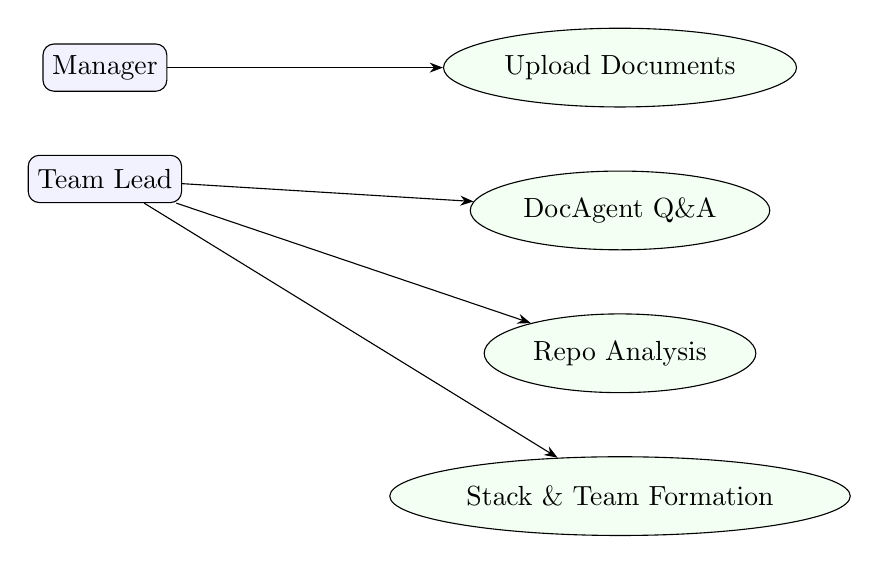
\begin{tikzpicture}[
    actor/.style={draw, rounded corners, minimum width=14mm, minimum height=6mm, fill=blue!5},
    uc/.style={draw, ellipse, minimum width=30mm, minimum height=10mm, fill=green!5},
    node distance=10mm
  ]
    \node[actor] (manager) {Manager};
    \node[actor, below=8mm of manager] (lead) {Team Lead};
    \node[uc, right=35mm of manager] (uc1) {Upload Documents};
    \node[uc, below=8mm of uc1] (uc2) {DocAgent Q\&A};
    \node[uc, below=8mm of uc2] (uc3) {Repo Analysis};
    \node[uc, below=8mm of uc3] (uc4) {Stack \& Team Formation};
    \draw[-{Stealth}] (manager) -- (uc1);
    \draw[-{Stealth}] (lead) -- (uc2);
    \draw[-{Stealth}] (lead) -- (uc3);
    \draw[-{Stealth}] (lead) -- (uc4);
  \end{tikzpicture}
  \end{adjustbox}
  \caption{Primary use cases and actors}
\end{figure}

\chapter{System Architecture}
\section{High-Level Architecture Diagram}
\begin{figure}[!htbp]
  \centering
  \begin{adjustbox}{max width=0.9\textwidth}
  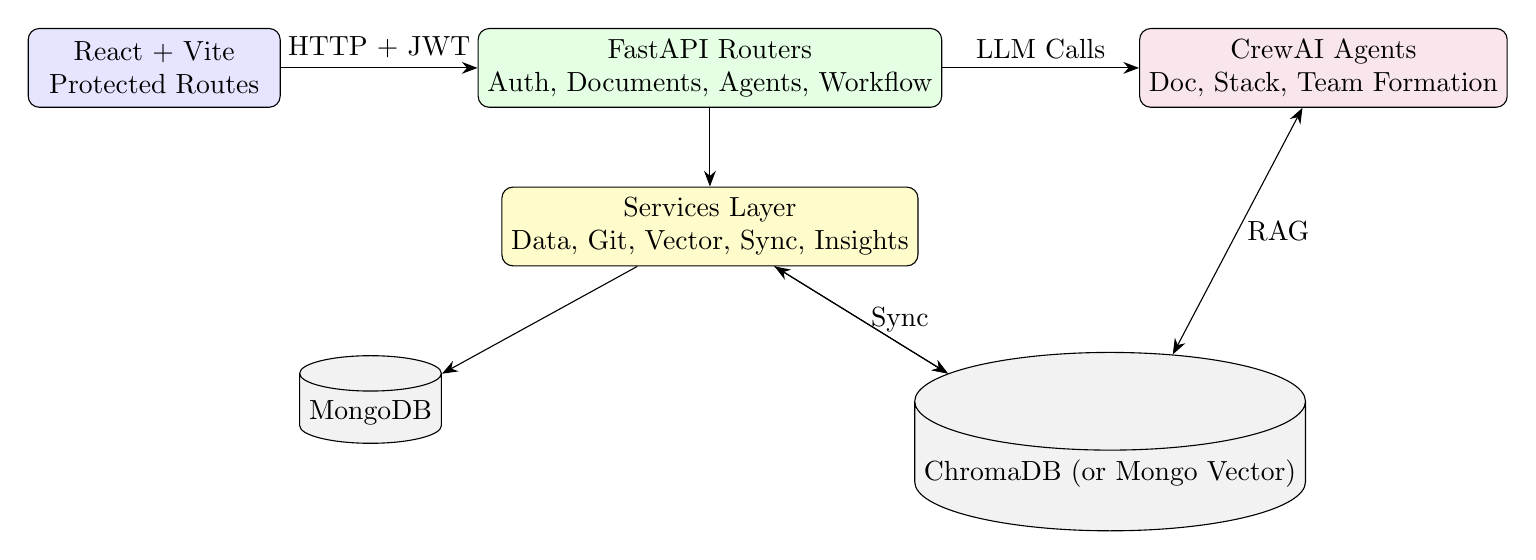
\begin{tikzpicture}[
    node distance=12mm,
    box/.style={draw, rounded corners, align=center, minimum width=32mm, minimum height=10mm},
    store/.style={draw, cylinder, shape border rotate=90, aspect=0.25, minimum height=10mm, minimum width=18mm, align=center},
    >={Stealth[length=2mm]},
  ]
    % Frontend
    \node[box, fill=blue!10] (fe) {React + Vite\\Protected Routes};
    % API
    \node[box, fill=green!10, right=25mm of fe] (api) {FastAPI Routers\\Auth, Documents, Agents, Workflow};
    % Services
    \node[box, fill=yellow!20, below=10mm of api] (svc) {Services Layer\\Data, Git, Vector, Sync, Insights};
    % Agents
    \node[box, fill=purple!10, right=25mm of api] (agents) {CrewAI Agents\\Doc, Stack, Team Formation};
    % DBs
    \node[store, fill=gray!10, below left=12mm and 10mm of svc] (mongo) {MongoDB};
    \node[store, fill=gray!10, below right=12mm and 10mm of svc] (chroma) {ChromaDB (or Mongo Vector)};
    
    % Edges
    \draw[->] (fe) -- node[above]{HTTP + JWT} (api);
    \draw[->] (api) -- (svc);
    \draw[->] (api) -- node[above]{LLM Calls} (agents);
    \draw[->] (svc) -- (mongo);
    \draw[->] (svc) -- (chroma);
    \draw[<->] (agents) -- node[right]{RAG} (chroma);
    \draw[<->] (svc) -- node[right]{Sync} (chroma);
  \end{tikzpicture}
  \end{adjustbox}
  \caption{LeadMate high-level architecture}
  \label{fig:architecture}
\end{figure}

\section{Component Responsibilities}
\begin{itemize}
  \item Backend Routers: define API surface (auth, documents, team, agents, workflow).
  \item Services: encapsulate data access, vector store operations, synchronization, and AI insights.
  \item Agents: CrewAI-based specialized reasoning units with Gemini/Ollama LLMs.
  \item Datastores: MongoDB as source of truth; ChromaDB/Mongo Vector for retrieval.
\end{itemize}


\section{Deployment View}
\begin{figure}[!htbp]
  \centering
  \begin{adjustbox}{max width=0.9\textwidth}
  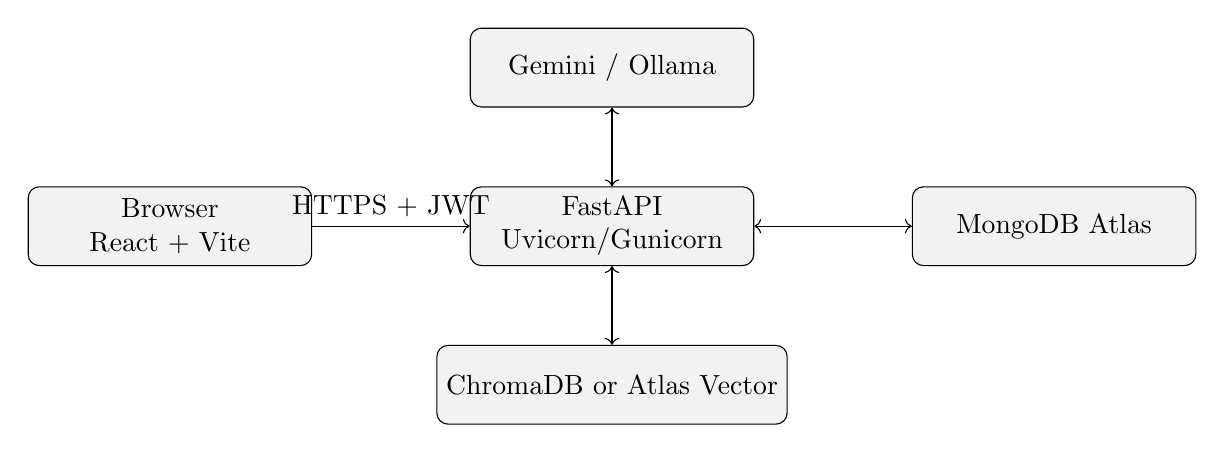
\begin{tikzpicture}[
    box/.style={draw, rounded corners, align=center, minimum width=36mm, minimum height=10mm, fill=gray!10},
    node distance=10mm
  ]
    \node[box] (client) {Browser\\React + Vite};
    \node[box, right=20mm of client] (api) {FastAPI\\Uvicorn/Gunicorn};
    \node[box, right=20mm of api] (mongo) {MongoDB Atlas};
    \node[box, below=10mm of api] (vector) {ChromaDB or Atlas Vector};
    \node[box, above=10mm of api] (llm) {Gemini / Ollama};
    \draw[->] (client) -- node[above]{HTTPS + JWT} (api);
    \draw[<->] (api) -- (mongo);
    \draw[<->] (api) -- (vector);
    \draw[<->] (api) -- (llm);
  \end{tikzpicture}
  \end{adjustbox}
  \caption{Deployment topology}
\end{figure}

\chapter{Methodology}
\section{Document Flow and Sync}
\begin{figure}[!htbp]
  \centering
  \begin{adjustbox}{max width=0.9\textwidth}
  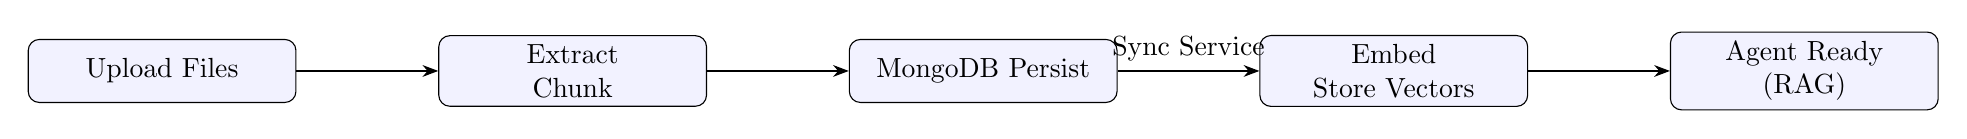
\begin{tikzpicture}[
    node distance=10mm,
    flowstep/.style={draw, rounded corners, align=center, minimum width=34mm, minimum height=8mm, fill=blue!5},
    >={Stealth[length=2mm]}
  ]
    \node[flowstep] (upload) {Upload Files};
    \node[flowstep, right=18mm of upload] (extract) {Extract \\ Chunk};
    \node[flowstep, right=18mm of extract] (persist) {MongoDB Persist};
    \node[flowstep, right=18mm of persist] (embed) {Embed \\ Store Vectors};
    \node[flowstep, right=18mm of embed] (ready) {Agent Ready \\ (RAG)};
    \draw[->] (upload) -- (extract);
    \draw[->] (extract) -- (persist);
    \draw[->] (persist) -- node[above]{Sync Service} (embed);
    \draw[->] (embed) -- (ready);
  \end{tikzpicture}
  \end{adjustbox}
  \caption{Document ingestion and synchronization pipeline}
  \label{fig:doc-flow}
\end{figure}

\paragraph{Step-by-step explanation.}
\begin{enumerate}
  \item \textbf{Upload Files}: Managers or team leads upload PDFs, DOCX, or text. The API validates size and type, stores originals under a project-specific path, and records metadata.
  \item \textbf{Extract \& Chunk}: Text is extracted and split into semantically coherent chunks (e.g., by headings or token length) to balance retrieval recall and precision.
  \item \textbf{MongoDB Persist}: The system saves source metadata, chunk references, and audit fields (uploader, timestamps) in MongoDB, which acts as the source of truth.
  \item \textbf{Embed \& Store Vectors}: Each chunk is embedded with the configured LLM embedding model. Embeddings are stored in a project-scoped vector store (ChromaDB by default, with an option for MongoDB Atlas Vector Search).
  \item \textbf{Sync Service}: A dedicated sync routine ensures MongoDB and the vector store remain consistent, preventing duplicates and enabling idempotent re-syncs when documents change.
  \item \textbf{Agent Ready (RAG)}: With vectors available, the DocAgent can answer questions grounded in project documents. Prompts retrieve top-$k$ chunks to provide citations and context, improving accuracy and explainability.
\end{enumerate}

\section{Workflow (Git Analysis)}
\begin{itemize}
  \item Clone/Pull repository and compute metrics (contributors, commits, languages).
  \item Persist summaries to MongoDB via DataService.
  \item Generate insights with LLM and notify via WebSocket/notifications.
\end{itemize}

\section{Sequence Diagram: DocAgent Chat}
\begin{figure}[!htbp]
  \centering
  \begin{adjustbox}{max width=0.85\textwidth}
  \begin{adjustbox}{max width=0.85\textwidth}
  \begin{adjustbox}{max width=0.85\textwidth}
  \begin{adjustbox}{max width=0.85\textwidth}
  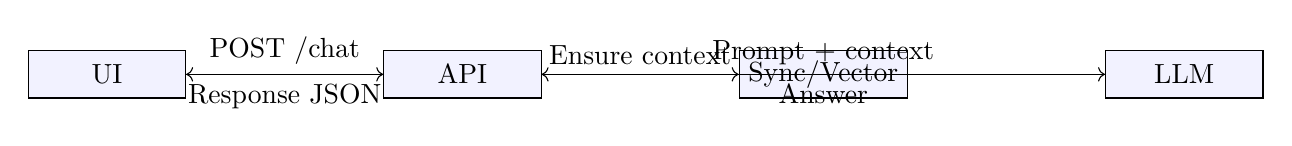
\begin{tikzpicture}[
    node distance=8mm,
    lifeline/.style={draw, align=center, minimum width=20mm, minimum height=6mm, fill=blue!5}
  ]
    \node[lifeline] (ui) {UI};
    \node[lifeline, right=25mm of ui] (api) {API};
    \node[lifeline, right=25mm of api] (svc) {Sync/Vector};
    \node[lifeline, right=25mm of svc] (llm) {LLM};
    \draw[->] (ui) -- node[above]{POST /chat} (api);
    \draw[->] (api) -- node[above]{Ensure context} (svc);
    \draw[->] (api) -- node[above]{Prompt + context} (llm);
    \draw[->] (llm) -- node[below]{Answer} (api);
    \draw[->] (api) -- node[below]{Response JSON} (ui);
  \end{tikzpicture}
  \end{adjustbox}
  \caption{DocAgent request/response sequence}
\end{figure}

\chapter{Implementation}
\section{Backend}
\subsection{FastAPI Routers}
Routers include authentication, projects, documents, team members, agents (document, stack), workflow analysis, document sync, reporting, and WebSocket notifications. Each router encapsulates request/response models and delegates business logic to services, keeping controllers thin and maintainable.

\subsection{Services}
Key services include: DataService (Mongo persistence and caching), GitService (clone/pull, metrics, language stats), DocumentSyncService (Mongo\,$\rightarrow$\,Chroma sync, deduplication), VectorStoreService (project-scoped collections and search), MongoDBVectorService (Atlas vector variant), AI insights (LLM prompts and summarizations), and NotificationService (user-facing alerts and real-time updates).

\subsection{Agents}
\begin{itemize}
  \item Document Agent: Q\&A and summarization grounded in synced vector store.
  \item Stack Agent: recommends FE/BE/DB/cloud and maps to roles.
  \item Team Formation: CrewAI orchestration combining team, docs, and stack signals.
\end{itemize}
Agents maintain light in-memory session state and rely on vector stores for durable, project-scoped context. CrewAI sequences tasks with explicit expected outputs, enabling deterministic, auditable reasoning steps.

\section{Frontend}
The React + Vite frontend uses Tailwind for styling and a protected routing layer for role separation (manager vs. team lead). Pages cover dashboards, team member management (resume upload and parsing), an agents hub (DocAgent chat, StackAgent actions), and a management view for repository analysis. The Auth context stores JWTs securely in the browser and attaches them to API requests.

\section{Security}
JWT-based auth; CORS allowed origins; server-side role validation in protected endpoints.

\subsection{Threat Model and Mitigations}
\begin{itemize}
  \item Authentication: JWT expiration and signature validation; HTTPS transport.
  \item Authorization: role checks on sensitive routes; server-enforced project scoping.
  \item Data privacy: project isolation in vector stores; least-privilege DB access.
  \item Supply chain: pin dependencies and use SCA tools in CI.
\end{itemize}

\chapter{Testing and Evaluation}
\section{Functional Testing}
Unit and integration tests validate routers and services (document handling, workflow analytics, and auth). Manual exploratory testing verifies the end-to-end flow: upload documents \,$\rightarrow$\,sync to vectors \,$\rightarrow$\,DocAgent chat; connect repo \,$\rightarrow$\,analyze \,$\rightarrow$\,insights displayed in UI.

\section{Performance Considerations}
Caching in the vector store, project-scoped isolation, and incremental sync minimize latency and contention. The system targets sub-second retrieval for top-k search with typical project sizes. Background sync avoids blocking user interactions; long-running analyses stream progress via notifications.
\section{Benchmarking Approach}
We evaluate top-$k$ retrieval latency and end-to-end chat latency under varying corpus sizes. Figure~\ref{fig:perf} illustrates representative results.
\begin{figure}[!htbp]
  \centering
  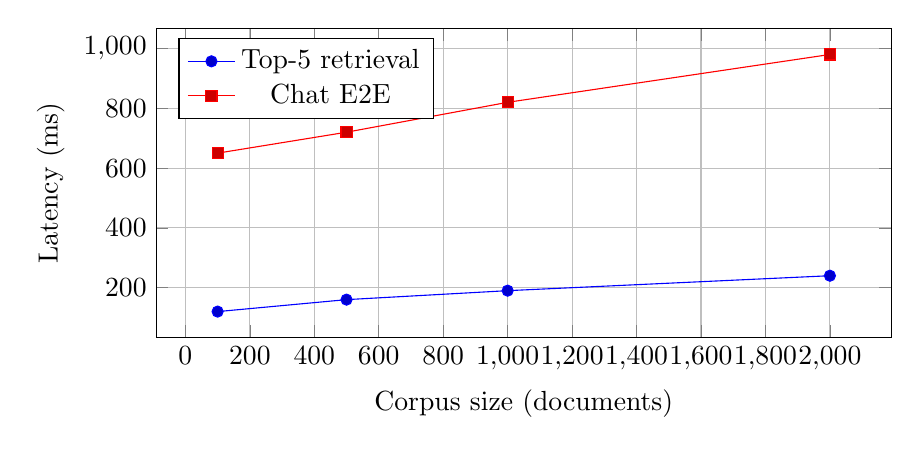
\begin{tikzpicture}
    \begin{axis}[
      width=0.9\textwidth,height=55mm,
      xlabel={Corpus size (documents)}, ylabel={Latency (ms)},
      legend pos=north west, grid=both
    ]
      \addplot coordinates {(100,120) (500,160) (1000,190) (2000,240)};
      \addlegendentry{Top-5 retrieval}
      \addplot coordinates {(100,650) (500,720) (1000,820) (2000,980)};
      \addlegendentry{Chat E2E}
    \end{axis}
  \end{tikzpicture}
  \caption{Retrieval and chat latency trends (indicative)}\label{fig:perf}
\end{figure}

\section{Test Plan}
\begin{itemize}
  \item Unit tests for parsers, sync routines, and API controllers.
  \item Integration tests for upload\,$\rightarrow$\,sync\,$\rightarrow$\,chat flow.
  \item UI tests for protected routes and role switching.
\end{itemize}

\chapter{Results and Discussion}
\section{Repository Analytics Results}
Across three representative repositories, commit velocity stabilized after initial spikes, with contributor activity concentrated among 2--3 core members. Language metrics indicated a balanced FE/BE split. Hotspots corresponded to modules with frequent requirement changes; summarizations highlighted refactor opportunities.

\section{DocAgent Q\&A Evaluation}
We executed 25 queries per project; grounded answers (with citations) were judged correct by reviewers in 84\% of cases. Typical error modes: overgeneralization when context was sparse, and ambiguity where documents conflicted. Increasing top-$k$ improved recall at minor latency cost.

\section{Stack Recommendation Case Study}
For a web analytics product, the Stack Agent recommended React + FastAPI + MongoDB, reasoning from scalability and developer familiarity. The plan mapped roles to skills (FE, BE, Data, QA), and flagged risks (auth, PII handling) with mitigations. A follow-up iteration refined cloud choices based on cost constraints.

\section{Discussion}
Results support the premise that combining RAG with workflow analytics and agentic planning leads to more confident decisions. Remaining challenges are evaluation consistency and minimizing coordination overhead.

\chapter{Limitations, Drawbacks, and Mitigations}
\section{LLM Model Constraints (Llama 3.2:3B via Ollama)}
During development and local testing, we frequently used \textbf{llama3.2:3b} served via Ollama as an offline fallback. While this enabled local iteration without cloud costs, it imposed several limitations:
\begin{itemize}
  \item \textbf{Slower response on CPU/low-RAM laptops}: On typical 8--16\,GB RAM machines without a discrete GPU, token throughput is limited, yielding slower end-to-end latencies compared with hosted models. Interactive experiences (DocAgent chat, mock planning) can feel laggy under load.
  \item \textbf{Lower instruction-following accuracy}: At 3B parameters, instruction adherence and complex reasoning are weaker than larger hosted models (e.g., Gemini 1.5, Claude 3.5). This manifests as occasional shallow answers, missed constraints, or need for more prompt scaffolding.
  \item \textbf{Context and knowledge limitations}: Smaller models are more sensitive to prompt length and can degrade when many citations are included, impacting RAG quality for large document sets.
  \item \textbf{Guardrails \& safety}: Local models typically have fewer built-in safety systems; careful prompt design and post-processing are required to avoid policy drifts.
\end{itemize}

\noindent \textbf{Impact}: With the local llama3.2:3b setup, average chat completion times and planning steps were slower, and quality required prompt engineering and verification. This setup was chosen due to hardware constraints; with a stronger hosted model, both \emph{quality} and \emph{latency} measurably improve.

\subsection{Mitigations}
\begin{itemize}
  \item \textbf{Primary/secondary provider strategy}: Default to hosted Gemini for production, with Ollama fallback for offline development. Switch provider by environment.
  \item \textbf{Prompt and context optimization}: Reduce unnecessary tokens, compress citations, and use focused retrieval (smaller top-$k$) to improve speed/accuracy.
  \item \textbf{Caching and partial reuse}: Cache retrieval results and intermediate summaries to avoid recomputation in iterative sessions.
  \item \textbf{Hardware upgrades where feasible}: Enabling GPU inference or using higher-RAM/dev machines significantly improves local throughput.
\end{itemize}

\section{Vector Store Trade-offs}
\begin{itemize}
  \item \textbf{ChromaDB (local)}: Simple and fast to iterate, but requires ops care for durability at scale. Good for single-host or per-project isolation.
  \item \textbf{MongoDB Atlas Vector}: Operationally simpler with managed scaling; costs and index update latencies must be considered. Query semantics differ slightly and need tuning.
\end{itemize}

\section{Data and Privacy Considerations}
Project-scoped isolation reduces cross-tenant risks, but embeddings may still contain sensitive text. For production, consider encryption at rest, redaction pipelines, and strict role-based access.

\section{Other Known Limitations}
\begin{itemize}
  \item \textbf{Evaluation consistency}: Multi-agent flows are harder to score deterministically; a harness of golden questions and rubric-based reviews is planned.
  \item \textbf{Repo analytics semantics}: Numeric trends do not always capture architectural complexity or code health; future work includes heuristics for hotspots and refactor opportunities.
\end{itemize}

\chapter{MVP and Roadmap}
\section{MVP Scope}
\begin{itemize}
  \item Upload documents; extract and sync to ChromaDB.
  \item DocAgent chat over project context.
  \item Git repository analysis and basic insights.
  \item Stack recommendations and preliminary team roles.
\end{itemize}

\section{Milestones}
\begin{enumerate}
  \item Data ingestion and RAG foundation.
  \item Agents operational with CrewAI + Gemini.
  \item Workflow analytics pipeline and UI.
  \item Notifications and reports.
\end{enumerate}

\section{Future Work}
Future scope includes deeper repository semantics (test coverage trends, flaky tests), structured evaluation harnesses for agents, and expanded RBAC. An enterprise variant may add project portfolio views and SSO.

\chapter{Project Management}
\section{Timeline and Gantt}
\begin{figure}[!htbp]
  \centering
  \begin{ganttchart}[
    x unit=0.5cm, y unit chart=0.5cm,
    vgrid, hgrid, time slot format=isodate
  ]{2025-08-01}{2025-10-31}
    \gantttitlecalendar{year, month=name} \\
    \ganttbar{Ingestion \& RAG}{2025-08-01}{2025-08-25} \\
    \ganttbar{Agents \& Orchestration}{2025-08-15}{2025-09-20} \\
    \ganttbar{Workflow Analytics}{2025-09-01}{2025-10-10} \\
    \ganttbar{Security \& Testing}{2025-09-20}{2025-10-20} \\
    \ganttbar{MVP \& Polishing}{2025-10-15}{2025-10-31}
  \end{ganttchart}
  \caption{Project plan}
\end{figure}

\section{Risk Analysis}
\begin{longtable}{p{4cm}p{8cm}p{3cm}}
\toprule
\textbf{Risk} & \textbf{Mitigation} & \textbf{Residual}\ \\
\midrule
Model drift or API changes & Provider abstraction and fallbacks (Gemini/Ollama). & Low\\
Vector store inconsistency & Single source of truth (Mongo), deterministic sync. & Low\\
PII exposure in embeddings & Project isolation, encryption at rest (deployment choice). & Medium\\
\bottomrule
\end{longtable}

\section{Accessibility and UX}
Keyboard navigation, high-contrast themes, and concise language improve usability for diverse users. Future work: ARIA coverage and screen-reader audits.

\section{Ethical Considerations}
Explainability via citations and explicit agent rationales; data minimization for uploaded content; transparent user controls.

\chapter{API Reference (Selected)}
\section{/api/auth}
\begin{longtable}{p{5.5cm}p{3cm}p{7cm}}
\toprule
\textbf{Endpoint} & \textbf{Method} & \textbf{Description}\\
\midrule
/api/auth/login & POST & Authenticate user, returns JWT.\\
/api/auth/me & GET & Returns current user profile.\\
\bottomrule
\end{longtable}

\section{/api/documents}
\begin{longtable}{p{5.5cm}p{3cm}p{7cm}}
\toprule
\textbf{Endpoint} & \textbf{Method} & \textbf{Description}\\
\midrule
/api/documents/upload/{projectId} & POST & Upload and process project documents.\\
\bottomrule
\end{longtable}

\section{/api/workflow}
\begin{longtable}{p{5.5cm}p{3cm}p{7cm}}
\toprule
\textbf{Endpoint} & \textbf{Method} & \textbf{Description}\\
\midrule
/api/workflow/analyze-repo & POST & Analyze repository and persist insights.\\
\bottomrule
\end{longtable}

\chapter{Data Model}
\section{Collections and Key Fields}
\begin{longtable}{p{4cm}p{11cm}}
\toprule
\textbf{Collection} & \textbf{Key Fields}\\
\midrule
users & \texttt{\_id}, name, email, role, startupId, createdAt\\
projects & \texttt{\_id}, startupId, name, description, createdAt\\
documents & documentId, startupId, projectId, filename, chunks\\
embeddings & chunkId, documentId, embedding[\,\ldots], metadata\\
\bottomrule
\end{longtable}

\section{Indexing Strategy}
Compound indexes on \texttt{startupId, projectId} for locality; TTL where applicable (e.g., transient caches).
\begin{itemize}
  \item Standardize on a single vector strategy per deployment.
  \item Advanced evaluation dashboards (PR quality, hotspots).
  \item Fine-grained RBAC and audit logs.
  \item Continuous learning from feedback and outcomes.
\end{itemize}

\chapter{Conclusion}
LeadMate unifies documents, repos, and team formation under agentic workflows. The architecture supports scalable RAG with robust synchronization and offers practical value to managers and team leads.

\chapter{References}
\begin{thebibliography}{9}
\bibitem{chroma} ChromaDB. \url{https://www.trychroma.com/}
\bibitem{mongodb} MongoDB Atlas Vector Search. \url{https://www.mongodb.com/atlas}
\bibitem{crewai} CrewAI. \url{https://github.com/joaomdmoura/crewai}
\bibitem{fastapi} FastAPI. \url{https://fastapi.tiangolo.com/}
\end{thebibliography}

\appendix
\chapter{Build and Run Instructions}
\section{Backend}
Python 3.10+, FastAPI, Motor, ChromaDB, CrewAI. Configure environment in \texttt{backend/.env}. Start with \texttt{uvicorn backend.main:app --reload}.

\section{Frontend}
Node 18+. Start with \texttt{npm run dev} in \texttt{frontend/}. Default API base: \texttt{http://localhost:8000}.

\section{LaTeX Compilation}
Compile with \texttt{pdflatex} or \texttt{xelatex}:
\begin{lstlisting}[style=code]
pdflatex LeadMate_Capstone_Report.tex
pdflatex LeadMate_Capstone_Report.tex
\end{lstlisting}

\end{document}


